\input{header.tex}

\subject{V 407}
\title{Fresnel'sche Formeln}
\date{%
  Durchführung: 03.05.2022
  \hspace{3em}
  Abgabe: 10.05.2022
}

\begin{document}

\maketitle
\thispagestyle{empty}
\tableofcontents
\newpage

\section{Zielsetzung}
\label{sec:Ziel}
Im folgenden Versuch sollen die diskreten Energiewerte der Elektronenhülle des Hg-Atoms untersucht werden. Dazu wird die integrale Energieverteilung
der beschleunigten Elektronen bei zwei unterschiedlichen Temperaturen untersucht. Anschließend werden für zwei weitere Temperaturen Franck-Hertz-Kurven aufgenommen.

\section{Theorie}
\label{sec:Theorie}

\noindent
Zur Strukturaufklärung der Elektronenhüllen werden Elektronenstoßexperimente durchgeführt. Dazu werden Elektronen mit geeigneter Energie auf Atome geschossen. Es wird
der dabei entstehende Energieverlust der Elektronen genutzt, Informationen über die Struktur zu erhalten.

\subsection{Aufbau und Ablauf des Franck-Hertz Experimentes}
\label{subsec:aufbau}
Die Franck-Hertz Apparatur ist schematisch in der \autoref{fig:franckAufb} dargestellt.

\begin{figure}[H]
    \centering
    \includegraphics[width=0.75\textwidth]{data/FranckHertz.png}
    \caption{Schematische Darstellung des Franck-Hertz Versuches \cite{Anleitung601}.}
    \label{fig:franckAufb}
\end{figure}

\noindent
Der Versuch besteht aus einem evakuierten Gefäß, in dem sich die auf die Struktur der Elektronenhülle zu untersuchende Probe befindet. In dem folgenden Versuch wird Quecksilber verwendet.
In der Glasglocke ist ein Draht angebracht, der aus einem hochschmelzenden Metall besteht. Dieser wird durch Gleichstrom erhitzt, weshalb infolge des glühelektrischen Effektes Elektronen austreten.
Der Glühdraht wird außerdem noch mit einem Oxid eines Erdalkalimetalls bestrichen, was die Austrittsarbeit $W$ herabsetzt. Die Austrittsarbeit ist dabei die für den Austritt von Elektronen benötigte Energie innerhalb einer Zeiteinheit.
Dadurch dass die Austrittsarbeit herabgesetzt wird, treten mehr Elektronen aus dem Draht.
Gegenüber der Heizelektrode ist eine Beschleunigungsanode, also eine gitterförmige, positiv geladenen Elektrode mit der Spannung $U_{\text B}$. Sie sorgt dafür, dass die Elektronen beschleunigt werden. Nach durchlaufen der Strecke zwischen dem Glühdraht und der Beschleunigungsanode
erhalten die Elektronen die kinetische Energie mit dem Betrag
\begin{align}
    \frac 12 m_0^2 v^2 = e_0 U_{\text B}.
    \label{eqn:beschlGl}
\end{align}
Dabei ist $e_0$ die Elementarladung, $m_0$ die Masse der Elektronen, $v_{\text vor}$ 
%Sicher, dass das vor der Beschleunigung die Geschwindigkeit ist? Wenn die Gleichung nur gültig ist wenn die 0 ist ist die gesamte Gleichung doch auch null. Außerdem ist die rechte Seite der Gleichung doch auch die Energie der Beschleunigungsanode??
die Geschwindigkeit vor der Beschleunigungsphase und $U_{\text B}$ die Beschleunigungsspannung.
Die Gleichung (\ref{eqn:beschlGl}) ist allerdings nur gültig, sofern die Geschwindigkeit der Elektronen zu Beginn der Beschleunigung null ist. \newline
Hinter der Beschleunigungsanode befindet sich die Auffängerelektrode, an der die auftreffenden Elektronen gemessen werden. Die Energiemessung geschieht über die Gegenfeldmethode, weshalb die Auffängerelektrode selbst auch eine geringe Gegenspannung $U_{\text A}$ besitzt.
Das dadurch entstehende Gegenfeld können nur die Elektronen durchlaufen, deren Geschwindigkeitskomponente in Feldrichtung $v_z$ die folgende Ungleichung erfüllt
\begin{align}
    \label{eqn:gegnFeldV}
    \frac 12 m_0 v_z^2 \geq e_0 U_{\text A}.
\end{align}
Im Beschleunigungsraum befinden sich demnach Hg-Atome, mit denen die Elektronen zusammenstoßen. Wenn die Energie der Elektronen nicht groß genug ist, führen sie elastische Stöße durch. Die Energieabgabe $\upDelta E$ an das Hg-Atom ist hier allerdings zu vernachlässigen, da der Massenunterschied zwischen den beiden
Stoßpartnern zu hoch ist. Sie beträgt
\begin{align}
    \upDelta E = \frac{4 m_0 M}{(m_0 + M)^2} \approx \SI{1,1 e-5}{\joule}.%1,1 \cdot 10^{-5}.
\end{align}
Die Richtungsänderungen der Elektronen ist allerdings für die Ergebnisse von großer Wichtigkeit. Darauf wird in \autoref{subsec:fehlerStoerung} nochmal eingegangen.
Die zweite Stoßmöglichkeit zwischen Elektronen und Hg-Atomen ist unelastisch. Wenn die Energie der Elektronen durch die Beschleunigung größer oder gleich groß der Energiedifferenz des ersten angeregten Zustandes und des Grundzustandes des Hg-Atoms ist, dann regt das Elektron dieses an.
Das Elektron gibt genau die Energie $\upDelta E = E_1 - E_0$ an die Atomhülle ab. Dabei bezeichnet $E_1$ die Energie des ersten Zustandes und $E_0$ die des Grundzustandes.
Das Hg-Atom ist nun in einem angeregten Zustand. Beim Übergang zurück in den Grundzustand emittiert es ein Lichtquant, also ein Photon, mit der Energie
\begin{align*}
    hf = E_1 - E_0.
\end{align*}
Die Frequenz wird mit $f$ bezeichnet und $h$ ist hierbei das Planck'sche Wirkungsquantum.
Wird die Beschleunigungsspannung $U_{\text B}$ kontinuierlich erhöht, treten auch mehr Stöße auf und die Elektronen besitzen nicht mehr genügend Energie, um gegen das Bremsfeld anzukommen.
Deshalb verringert sich der Auffängerstrom $I_{\text A}$ über den zeitlichen Verlauf gesehen immer wieder und es ergibt sich der Kurvenverlauf, der aus \autoref{fig:franckVerlauf} abzulesen ist.
Die Abstände zwischen den einzelnen Peaks $U_n$ ist über die folgende Relation zu berechnen.
\begin{align}
    U_n = \frac{1}{e_0} (E_n - U_{n-1}).
    \label{eqn:abstMaxima}
\end{align}
Dabei bezeichnet $U_n$ den Abstand zweier aufeinander folgender Maxima und analog dazu $E_n$ und $E_{n-1}$ die Anregungspotentiale der Elektronenhülle.

\begin{figure}[H]
    \centering
    \includegraphics[width=0.75\textwidth]{data/VerlaufFH.png}
    \caption{Kurvenverlauf des Auffängerstromes $I_{\text A}$ gegen die Bremsspannung $U_{\text B}$ \cite{Anleitung601}.}
    \label{fig:franckVerlauf}
\end{figure}

\subsection{Fehlerquellen und Störungen}
\label{subsec:fehlerStoerung}

Die Ergebnisse aus dem Versuch werden allerdings nicht die ideale Franck-Hertz Kurve ergeben, wie sie in \autoref{fig:franckVerlauf} abgebildet ist. Die Gründe für mögliche Störungen und erwartbare Fehlerquellen werden im Folgenden dargestellt. \newline
Der erste Grund ist auf den Einfluss des Kontaktpotentials zurückzuführen. Das Beschleunigungspotential zwischen dem Glühdraht und der Beschleunigungsanode ist von der von außen angelegten Spannung verschieden, da die Elektroden aus unterschiedlichen Materialien bestehen.
Durch die unterschiedlichen Materialien haben die Elektroden auch unterschiedliche Austrittsarbeiten für die Elektronen und das tatsächliche Beschleunigungspotential $U_{\text {B, eff}}$ ist definiert zu
\begin{align}
    U_{\text {B, eff}} = U_{\text B} - \frac{1}{e_0} (\phi_{\text B} - \phi_{\text G}).
    \label{eqn:potentialGef}
\end{align}
Wobei der Ausdruck
\begin{align}
    K = \frac{1}{e_0} (\phi_{\text B} - \phi_{\text G})
\end{align}
das Kontaktpotential ist, $\phi_{\text G}$ die Austrittsarbeit aus dem Glühdraht und $\phi_{\text B}$ die Austrittsarbeit aus der Beschleunigungselektrode ist.
Das Potentialgefälle ist außerdem durch die \autoref{fig:poteGef} verbildlicht.

\begin{figure}[H]
    \centering
    \includegraphics[width=0.75\textwidth]{data/potentialgefälle.png}
    \caption{Die Potentialverhätlnisse zwischen dem Glühdraht und der Beschleunigungsanode \cite{Anleitung601}.}
    \label{fig:poteGef}
\end{figure}

\noindent
Der zweite Grund für die Abweichungen zu der idealen Kurve ist das Energiespektrum der Elektronen. Beim Austreten der Elektronen aus dem Glühdraht durch den glühelektrischen Effekt haben die Elektronen nicht alle die gleiche Anfangsgeschwindigkeit.
Nach der Beschleunigungsphase haben sie somit eine Energieverteilung, die bei $U_{\text{B, eff}}$ beginnt und kontinuierlich steigt. Somit setzen die unelastischen Stöße nicht bei einer genau definierten Beschleunigungsspannung ein und sind stattdessen über einen gewissen Bereich verteilt.
Die Kurve fällt deshalb nach einem Maximum nicht auf den Wert null herab, sondern sinkt auf ein gewisses Stromminimum herab. \newline
Außerdem ist der Einfluss der elastischen Zusammenstöße zwischen Elektronen und Atomen zu nennen. Diese führen, wie bereits erwähnt, zwar nicht zu merklichen Energieabnahmen, jedoch ändern sie die Richtung der Elektronen beträchtlich.
Finden diese im Raum zwischen Kathode und Beschleunigungsanode statt, dann tragen sie nicht wesentlich zur Franck-Hertz Kurve bei. Im Raumbereich zwischen der Beschleunigungs- und der Auffängerelektrode führen sie dazu, dass die Verteilung der z-Komponente der Geschwindigkeiten und somit die Franck-Hertz Kurve abflacht und verbreitert. \newline
Da für die Beobachtung der Kurve Zusammenstöße zwischen Elektronen und Hg-Atomen notwendig sind, nimmt der Dampfdruck des zu untersuchenden Stoffes Einfluss auf ebendiese Kurve.
Es wird die mittlere freie Weglänge $\overline w$ der Atome klein gegen den Abstand $a$ zwischen Kathode und Beschleunigungselektrode gewählt und somit die Wahrscheinlichkeit der Zusammenstöße erhöht. Die Weglänge $\overline w$ kann über den Druck $p_{\text{sät}}$
in der Glasglocke genau eingestellt werden und es folgt mit
\begin{align*}
    \overline w \, [\si{\centi\meter}] = \frac{0,0029}{p_{\text{sät}}} \, [\si{\milli\bar}]
\end{align*}
ein Zusammenhang zwischen dem Sättigungsdampfdruck $p_{\text{sät}}$ und der Temperatur $T$
\begin{align}
    p_{\text{sät}}(T) = 5,5\cdot 10^{7} \text e^{\frac{-6876}{T}}.
\end{align}
Es muss $\overline w$ etwa um $1000$ bis $4000$ mal kleiner eingestellt werden, als $a$. In der verwendeten Apparatur beträgt $a$ etwa $\SI{1}{\centi\meter}$.
\section{Durchführung}
\label{sec:Durchführung}

Für den Versuch wird der in \autoref{fig:messapp} dargestellte Aufbau verwendet, wobei der He-Ne-Laser nicht um die Strahlachse schwenkbar war.

\begin{figure}[H]
	\centering
	\includegraphics[width=0.6\linewidth]{data/v407Messapparatur.jpg}
	\caption{Schematische Darstellung der verwendeten Messapparatur.\cite{Anleitung407}}
	\label{fig:messapp}
\end{figure}

\noindent
Bevor die eigentliche Messung beginnen kann, muss zunächst die Messapparatur justiert werden.
Es wird hierfür der Silizium-Spiegel entfernt und eine Messung der Intensität des Laser-Strahles durchgeführt. Anschließend wird der Spiegel erneut auf dem Probehalter montiert
und so ausgerichtet, dass der Laser-Strahl dierekt auf den Laserkopf zurück reflektiert wird. Auch wird darauf geachtet, dass das Goniometer in dieser Stellung genau einen Winkel
von 0° zeigt, um später die Abweichung des Winkels zu dieser Stellung abzulesen. Anschließend ist die Justierung abgeschlosssen und die Mesung kann beginnen.
\newline\newline
Für die eigentliche Messung wird zunächst ein Winkel für die Polarisation eingestellt. Es wurden zwei Messreihen mit einem Polarisationswinkel von 0° und 90° durchgeführt.
Im Anschluss wird die Intensität des reflektierten Laserstrahles für unterschiedliche Eintrittswinkel des Lasers auf den Silizium-Spiegel gemessen. Es werden dabei Winkel in
einem Intervall von 10° bis 88° gemessen, da für Winkel unter 10° und über 88° die Messapparatur den Laser blockiert. Die Messwerte werden dabei jeweils in einem Abstand
von 2° aufgenommen.
\section{Auswertung}
\label{sec:Auswertung}

\subsection{Zählrohr-Charakteristik}

Die gemessenen Werte zur Bestimmung der Charakteristik sind in \autoref{tab:messw} zu finden.
\begin{table}[H]
  \caption{Messwerte zur Zählrohr-Charakteristik.}
  \label{tab:messw}
  \centering
  \begin{tabular}{c c c c}
      \toprule
      U [$\si{\volt}$] & N [Imp/$\SI{120}{\second}$] & U [$\si{\volt}$] & N [Imp/$\SI{120}{\second}$] \\
      \midrule
      320 & $ 11680 \pm 108 $ & 520 & $ 12344 \pm 111$ \\
      330 & $ 11939 \pm 109 $ & 530 & $ 12406 \pm 111$ \\
      340 & $ 11946 \pm 109 $ & 540 & $ 12626 \pm 112$ \\
      350 & $ 12320 \pm 111 $ & 550 & $ 12504 \pm 112$ \\
      360 & $ 12291 \pm 111 $ & 560 & $ 12545 \pm 112$ \\
      370 & $ 12371 \pm 111 $ & 570 & $ 12832 \pm 113$ \\
      380 & $ 12393 \pm 111 $ & 580 & $ 12695 \pm 113$ \\
      390 & $ 12433 \pm 112 $ & 590 & $ 12612 \pm 112$ \\
      400 & $ 12259 \pm 111 $ & 600 & $ 12620 \pm 112$ \\
      410 & $ 12157 \pm 110 $ & 610 & $ 12574 \pm 112$ \\
      420 & $ 12428 \pm 111 $ & 620 & $ 12907 \pm 114$ \\
      430 & $ 12475 \pm 112 $ & 630 & $ 12812 \pm 113$ \\
      440 & $ 12566 \pm 112 $ & 640 & $ 12769 \pm 113$ \\
      450 & $ 12440 \pm 112 $ & 650 & $ 12848 \pm 113$ \\
      460 & $ 12645 \pm 112 $ & 660 & $ 12977 \pm 114$ \\
      470 & $ 12446 \pm 112 $ & 670 & $ 13033 \pm 114$ \\
      480 & $ 12625 \pm 112 $ & 680 & $ 13026.\pm 114$ \\
      490 & $ 12516 \pm 112 $ & 690 & $ 13363.\pm 116$ \\
      500 & $ 12415 \pm 111 $ & 700 & $ 13219.\pm 115$ \\
      510 & $ 12632 \pm 112 $ &       &                \\
      \bottomrule
    \end{tabular}
\end{table}

Die Charakteristik ist zusammen mit einer Ausgleichsgeraden für die Werte des Plateau-Bereichs in \autoref{fig:plot} dargestellt. Der Plateau-Bereich wurde hierfür
von $\SI{420}{\volt}$ bis $\SI{560}{\volt}$ gewählt.\\
Da die Werte der Zählrate Poison-verteilt sind, ist ihr Fehler $\Delta N$ als $\sqrt{N}$ anzunehmen.

\begin{figure}[H]
  \centering
  \includegraphics{plot2.pdf}
  \caption{Teilchenanzahl in Abhängigkeit der Spannung.}
  \label{fig:plot}
\end{figure}


Für die Ausgleichsgerade der Form $y = a \cdot x + b$ ergeben sich die Werte
\begin{align*}
  a &= (0,14 \pm 0,5927) \frac{1}{\si{\volt}} \\
  b &= (12434 \pm 291,53)
\end{align*}





Die Plateausteigung ist durch
\begin{equation*}
  N_\text{rel} = \frac{100a}{N(U_\text{m})}
\end{equation*}
gegeben, wobei $U_\text{m}$ als mittlerer Plateauwert gewählt wird.

Der Fehler der Plateausteigung kann über die Gauß'sche Fehlerfortpflanzug zu
\begin{equation*}
  \Delta N_\text{rel} = \sqrt{\left(\frac{100}{N}\symup{\Delta}a\right)^2 + \left(\frac{100a}{N^2} \symup{\Delta}N\right)^2}
\end{equation*}
bestimmt werden.






Daraus ergibt sich eine Plateau-Steigerung von
\begin{align*}
  N_\text{rel} &= \SI{0,11+-0,47}{\percent\per100\volt}
\end{align*}


\subsection{Totzeit}

Zur Bestimmung der Totzeit wurde, wie im vorherigen Abschnitt erwähnt, ein Oszilloskop verwendet. Das Ergebniss ist in \autoref{fig:osz} zu sehen.
\begin{figure}[H]
  \centering
  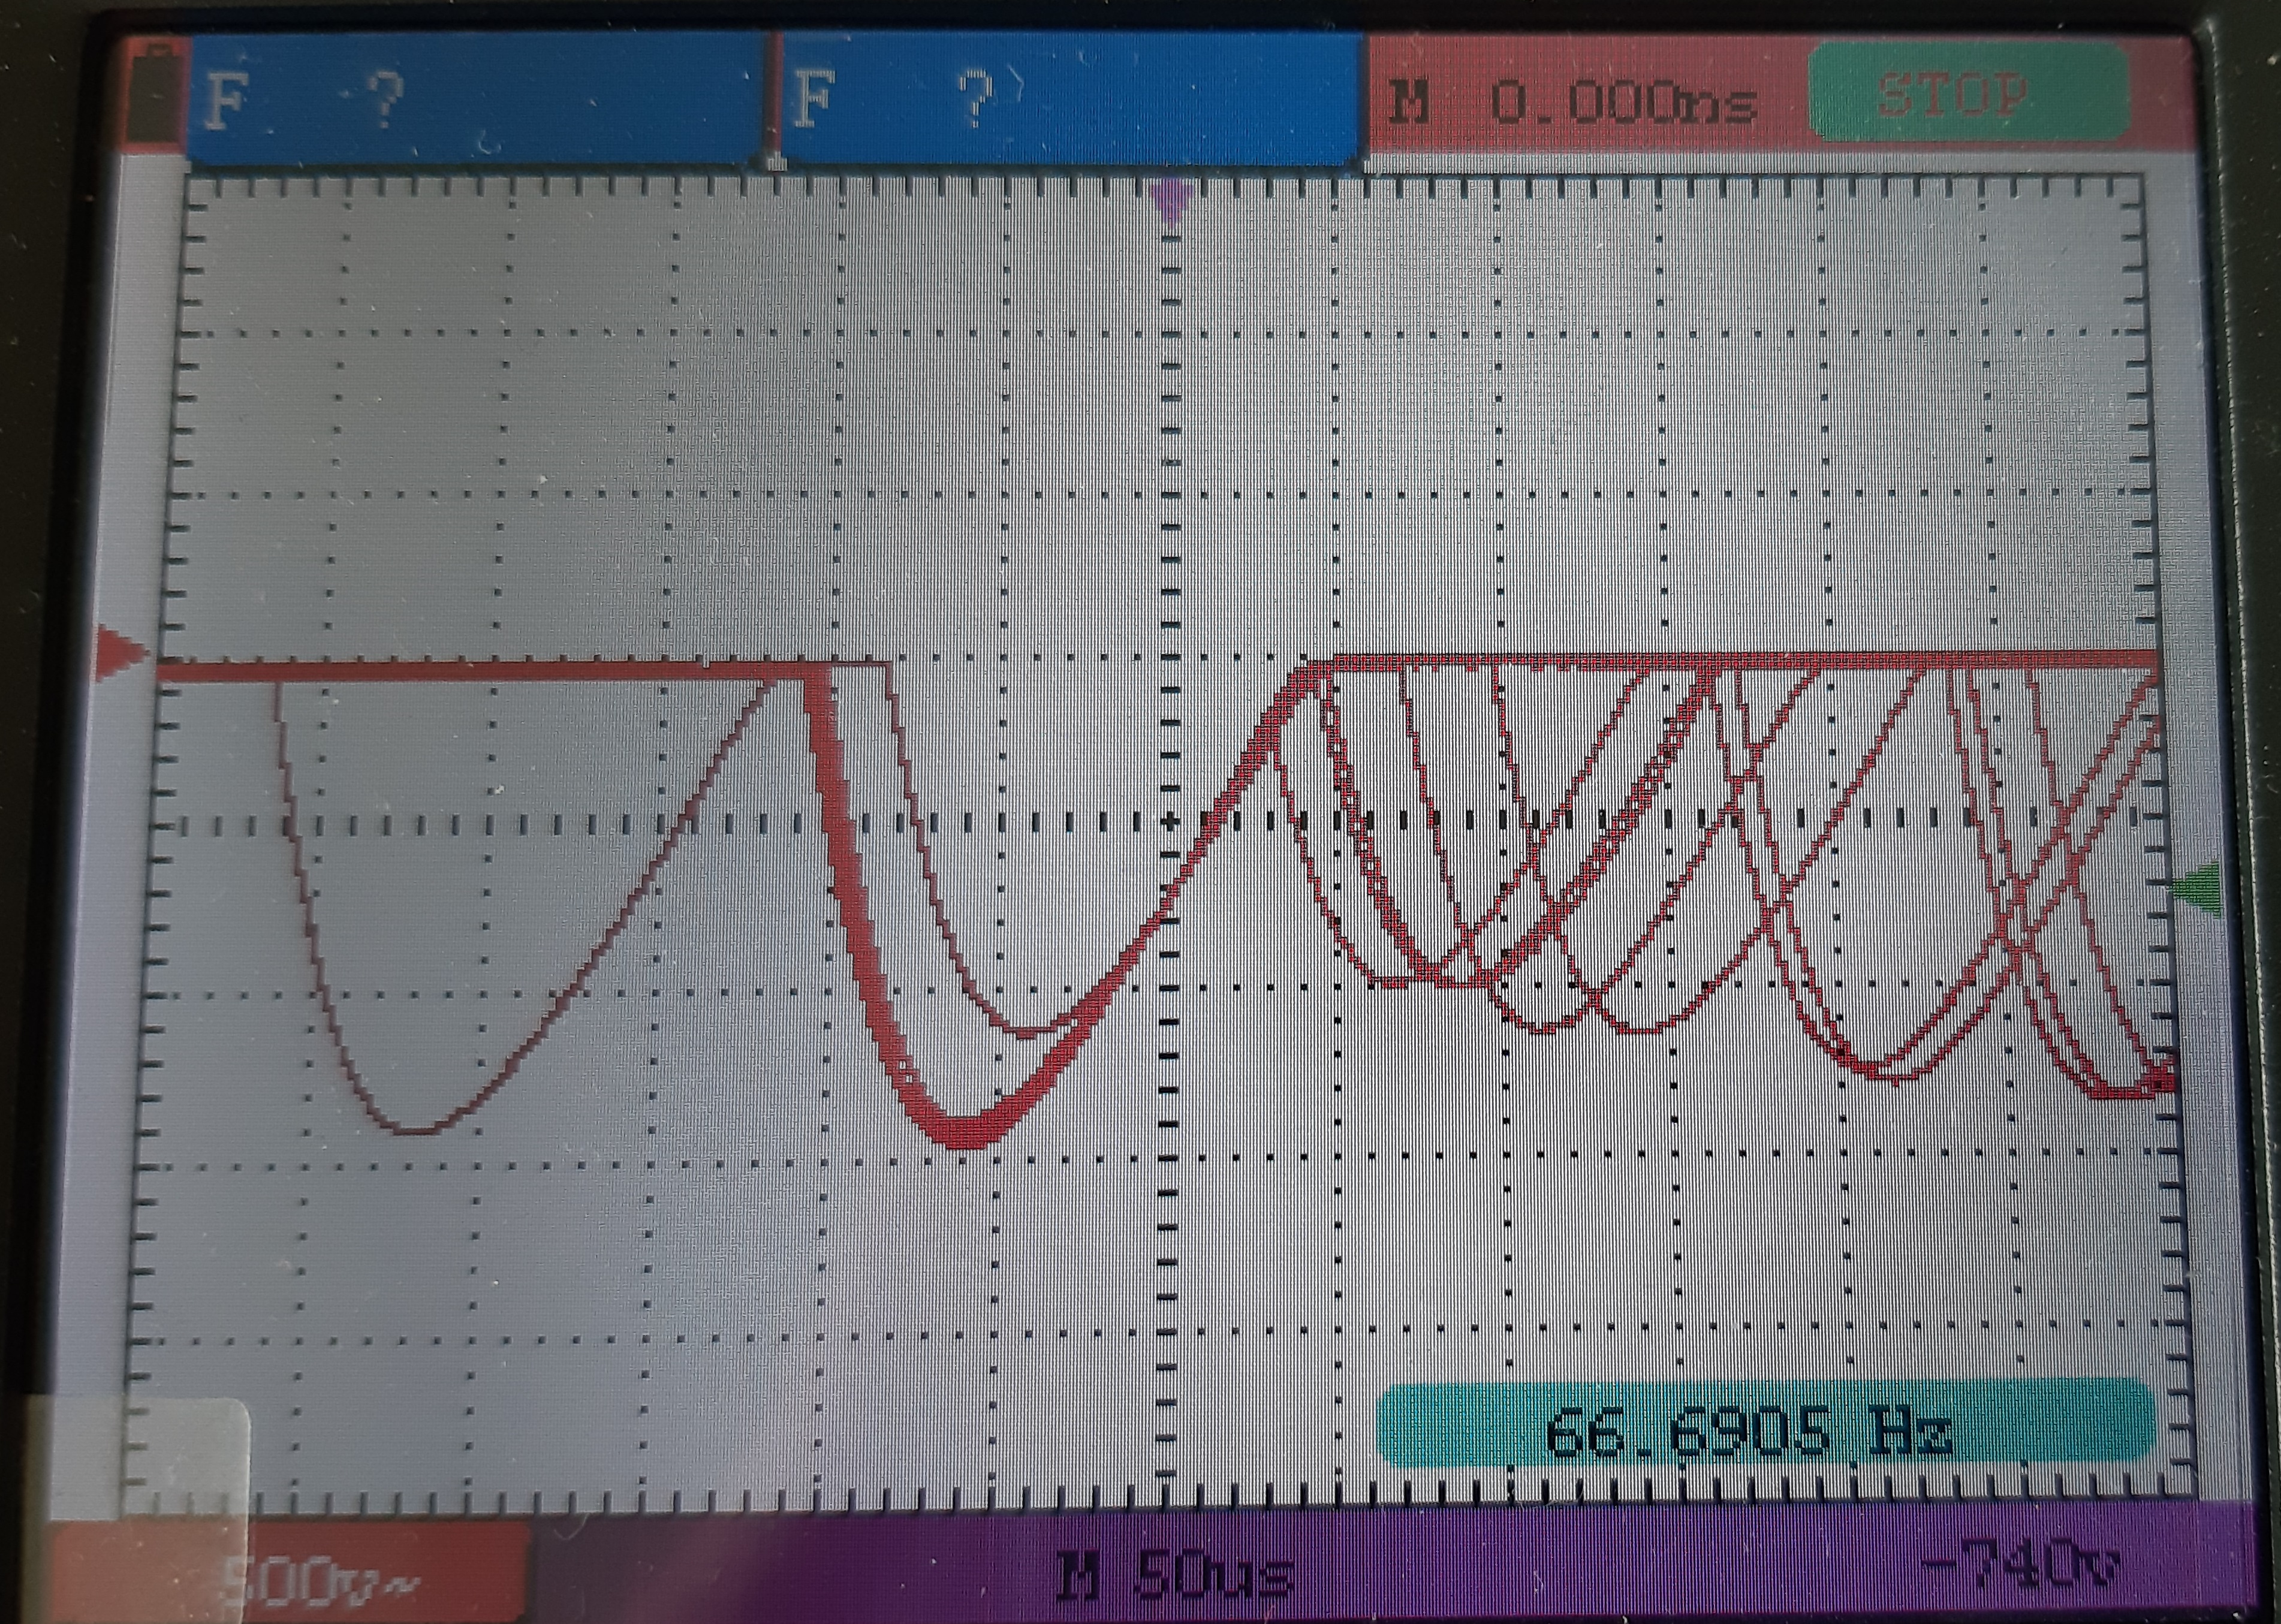
\includegraphics[width=0.7\textwidth]{data/zkurve.jpg}
  \caption{Ergebnisse der Messung mit dem Oszilloskop.}
  \label{fig:osz}
\end{figure}

Die Totzeit kann durch Ablesen bestimmt werden zu
\begin{align*}
  T_\text{t} &= (110 \pm 10) \si{\micro\second}, \\
\end{align*}
die Nachladung zu
\begin{align*}
  T_{n} &= (130 \pm 10) \si{\micro\second}, \\
\end{align*}



Die Totzeit wurde ebenfalls mittels der Zwei-Quellen-Methode bestimmt. Die Ergebnisse der Messungen mit dem ersten Präparat $N_1$, die mit beiden Präparaten
$N_{1+2}$ und die nur mit dem zweiten $N_2$ sind im Folgenden aufgeführt.

\begin{align*}
  N_1 &= 19.344 \pm 139 \\
  N_{1+2} &= 34.387 \pm 185 \\
  N_2 &= 15.440 \pm 124 \\
\end{align*}

Mit Hilfe von Gleichung \eqref{eqn:tot} kann nun die Totzeit zu
\begin{align*}
  T \approx (79,75 \pm 0,30)\si{\micro\second} \\
\end{align*}

bestimmt werden.
Der Fehler wurde dabei mit der Gleichung
\begin{equation*}
  \symup{\Delta}T = \sqrt{\left(\frac{N_1 - N_{1+2}}{2N_2 N_1^2} \cdot \symup{\Delta}N_1 \right)^2 + \left(\frac{N_{1+2} - N_{1}}{2N_1 N_2^2} \cdot \symup{\Delta}N_2 \right)^2
  + \left( \frac{\symup{\Delta}N_{1+2}}{2N_1 N_2}\right)^2} 
\end{equation*}
berechnet.

\subsection{Freigesetzte Ladung pro Teilchen}

Beim Aufnehmen der Messwerte für die Bestimmung der Charakteristik wurden nebenher die jeweils zu den Spannungen zugehörigen Zählrohrströme gemessen. Mit Hilfe von
Gleichung \eqref{eqn:ener} lässt sich daraus die pro Teilchen freigesetze Ladungsmenge $\Delta Q$ berechnen. Die Messwerte sind zusammen mit den errechneten Ladugsmengen in
\autoref{tab:lad} aufgeführt.
\newline
Der Fehler von $\Delta Q$ ist dabei gegene durch
\begin{equation*}
  \Delta (\Delta Q) = \sqrt{\left(\frac{t}{N} \cdot \Delta I \right)^2 + \left(\frac{I \cdot t}{N^2} \cdot \Delta Z\right)^2}.
\end{equation*}

\begin{table}[H]
  \caption{Werte der Regression vom Grad drei.}
  \label{tab:lad}
  \centering
  \begin{tabular}{c c c c c}
      \toprule
      U [$\si{\volt}$] & N [Imp/$\si{\second}$] & I [$\si{\micro\ampere}$] & $\Delta Q$ [$10^9 \si{\coulomb}$] & $10^{10} \frac{\Delta Q}{e}$ \\
      \midrule
      350 & $ 12320 \pm 111 $ & $ 0,2 \pm 0,05 $ & $ 1,95 \pm 0,487 $ & $ 1,22 $ \\
      450 & $ 12440 \pm 112 $ & $ 0,3 \pm 0,05 $ & $ 2,89 \pm 0,483 $ & $ 1,80 $ \\
      540 & $ 12626 \pm 112 $ & $ 0,4 \pm 0,05 $ & $ 3,80 \pm 0,476 $ & $ 2,37 $ \\
      580 & $ 12695 \pm 113 $ & $ 0,5 \pm 0,05 $ & $ 4,73 \pm 0,474 $ & $ 2,95 $ \\
      670 & $ 13033 \pm 114 $ & $ 0,6 \pm 0,05 $ & $ 5,52 \pm 0,463 $ & $ 3,45 $ \\
      700 & $ 13219 \pm 115 $ & $ 0,7 \pm 0,05 $ & $ 6,35 \pm 0,457 $ & $ 3,96 $ \\
      \bottomrule
    \end{tabular}
\end{table}

Nun kann die Ladungsmenge gegen die zugehörige Spannung aufgetragen werden.

\begin{figure}[H]
  \centering
  \includegraphics{plot2.pdf}
  \caption{Ladungsmenge in Abhängigkeit der Spannung.}
  \label{fig:plot}
\end{figure}

Die lineare Regression der Form $y = m \cdot x + b$ liefert die Werte
\begin{align*}
  a &= (12,31 \pm 0,87) \cdot 10^{-3} \si{\coulomb\per\volt} \\
  b &= (-2,54 \pm 0,49) \si{\coulomb}.
\end{align*}

\section{Diskussion}
\label{sec:Diskussion}
Abschließend lässt sich feststellen, dass die meisten Messungen sehr präzise sind und nur geringe Fehler aufweisen. Die einziege größere Unsicherheit bei der Messung war das
Stoppen der Fallzeit im Viskosimeter per Stoppuhr. Diese wurde jedoch augenscheinlich durch viele Messungen und Mittelung der Werte gut ausgeschaltet.

Trotz dessen weicht der Wert für die Viskosität von Wasser bei Raumtemperatur um 0,5\% vom Literaturwert ab.


\section{Anhang}
\label{sec:Anhang}

\begin{figure}[H]
    \centering
    \includegraphics[width=0.5\textwidth]{Dateien/V107daten1.jpg}
    \caption{Originale Messdaten.}
    \label{fig:origDaten1}
\end{figure}
\begin{figure}[H]
    \centering
    \includegraphics[width=0.5\textwidth]{Dateien/V107daten2.jpg}
    \caption{Originale Messdaten.}
    \label{fig:origDaten2}
\end{figure}

\printbibliography{}

\addsec*{Anhang}{
  \begin{figure}[H]
    \centering
    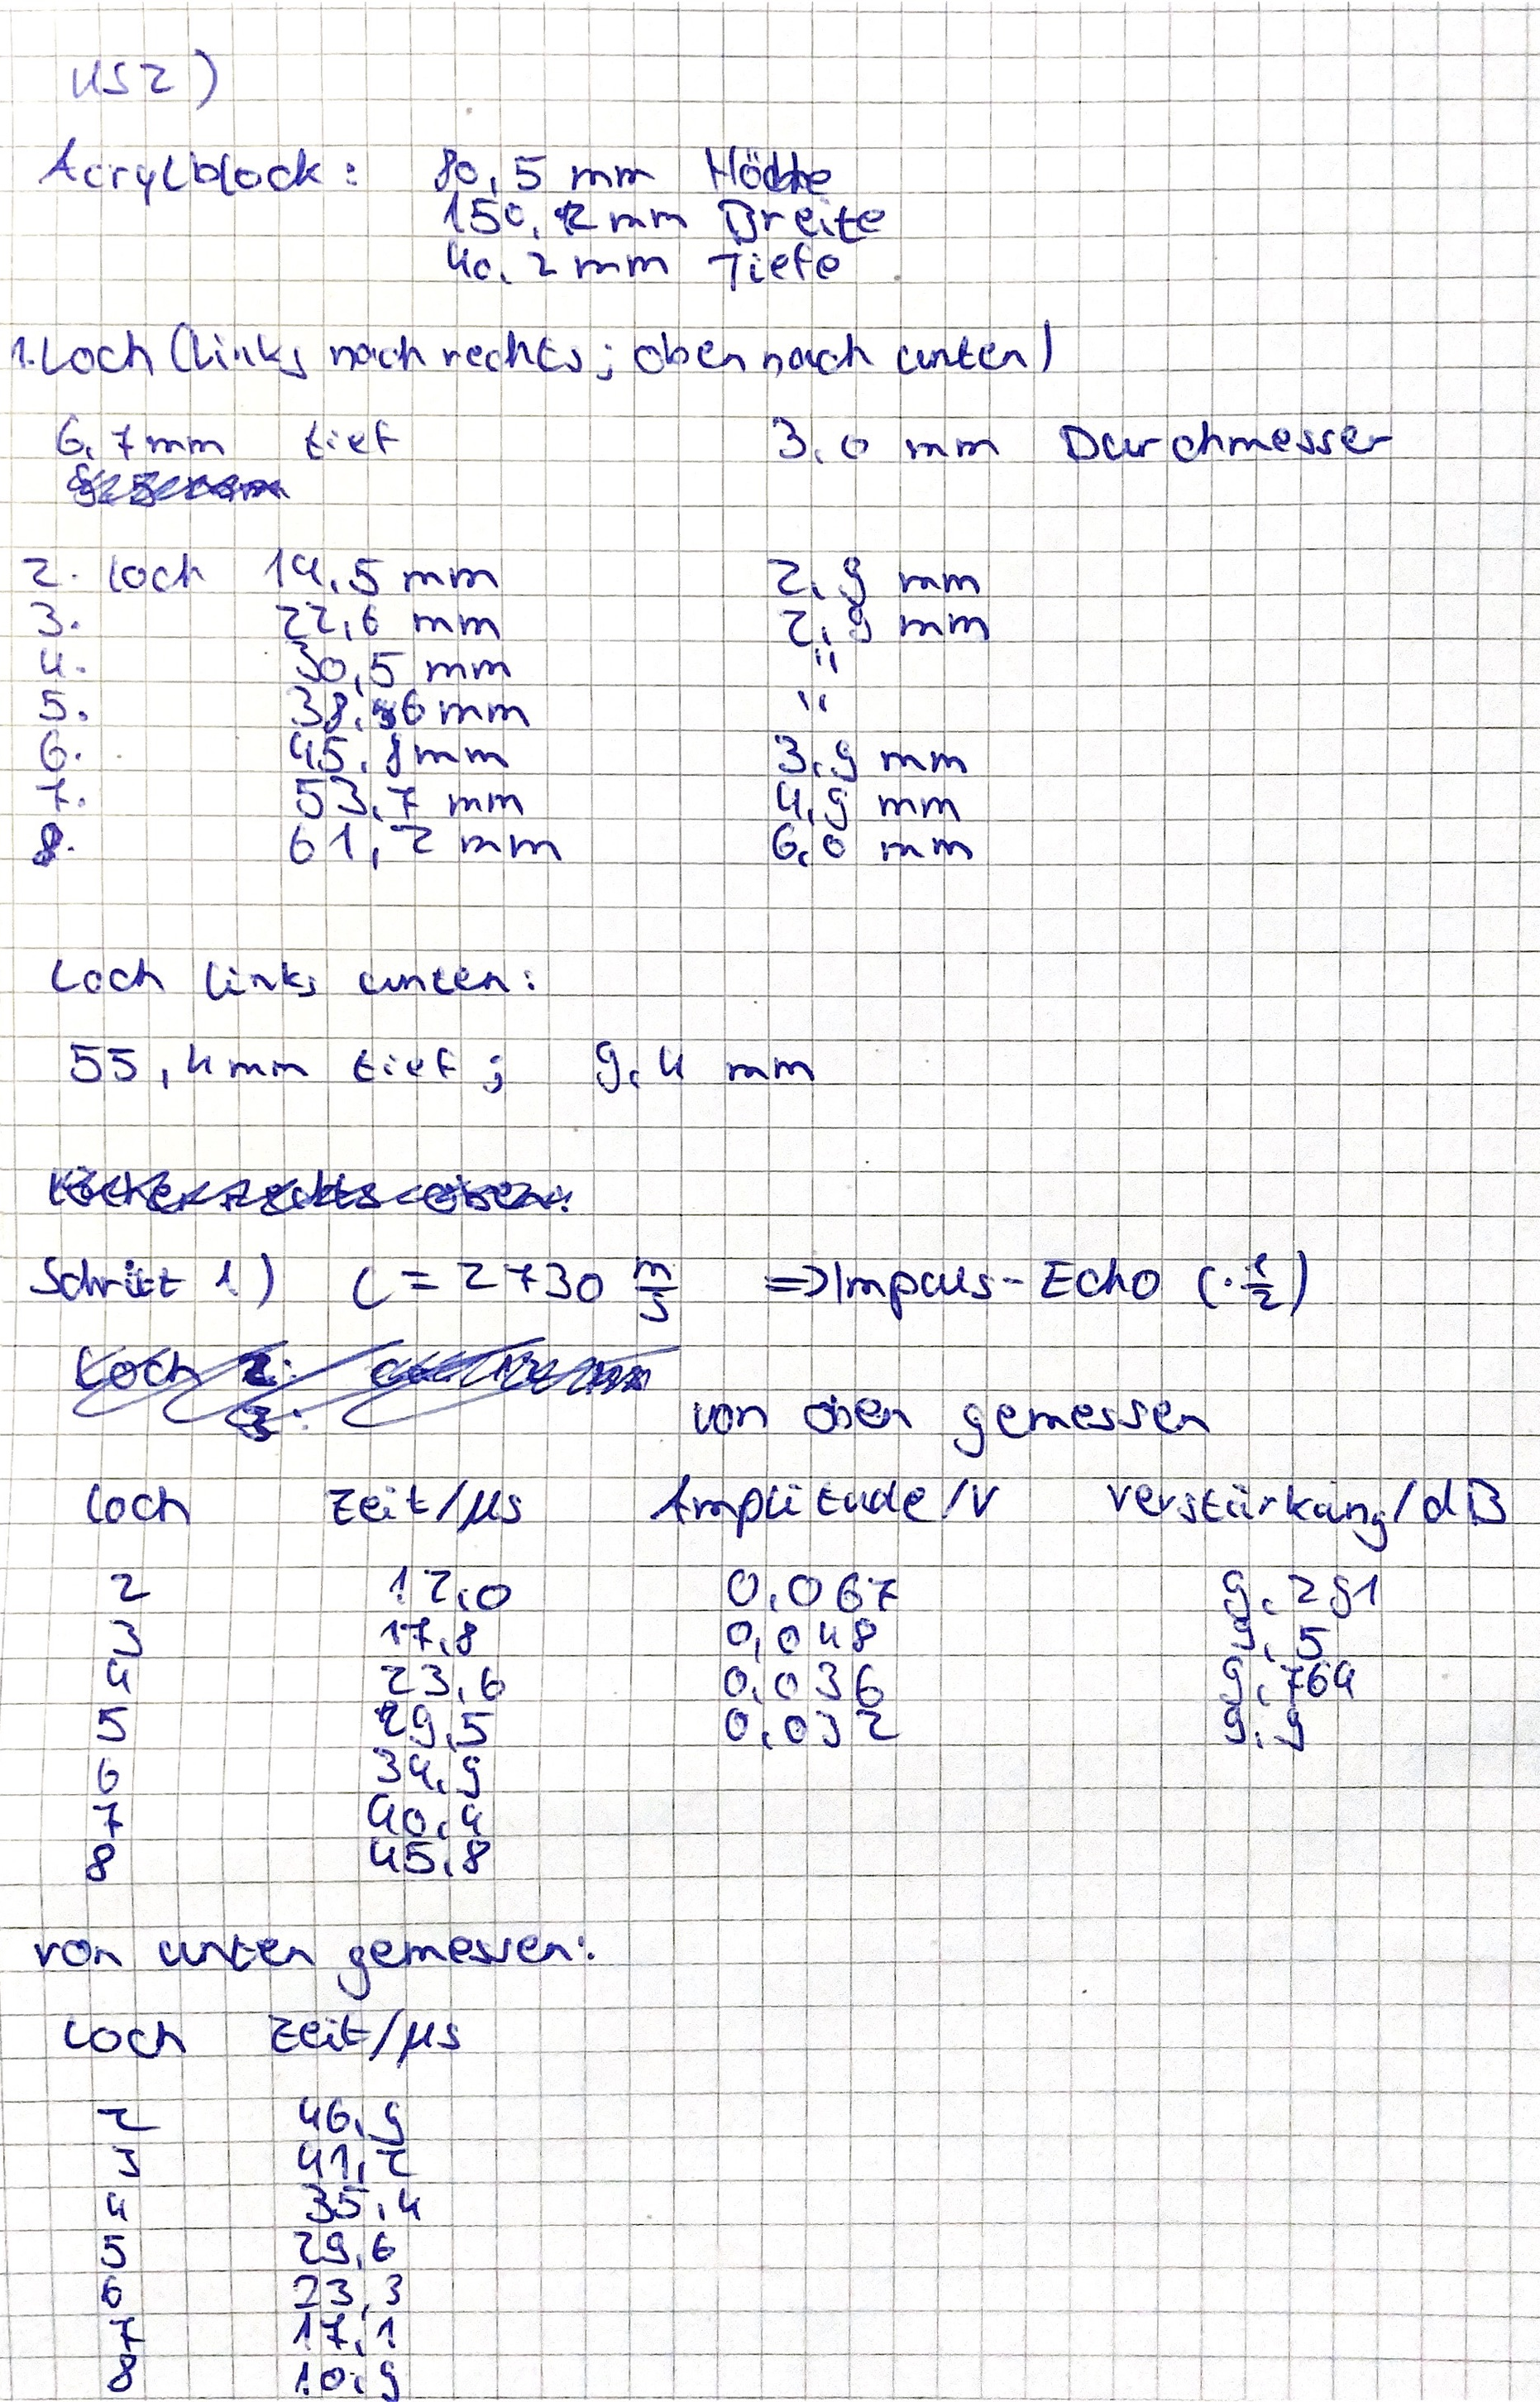
\includegraphics[width=0.75\textwidth]{data/origDaten1.png}
    \caption{Originale Messdaten.}
    \label{fig:origDaten1}
  \end{figure}
  \begin{figure}[H]
    \centering
    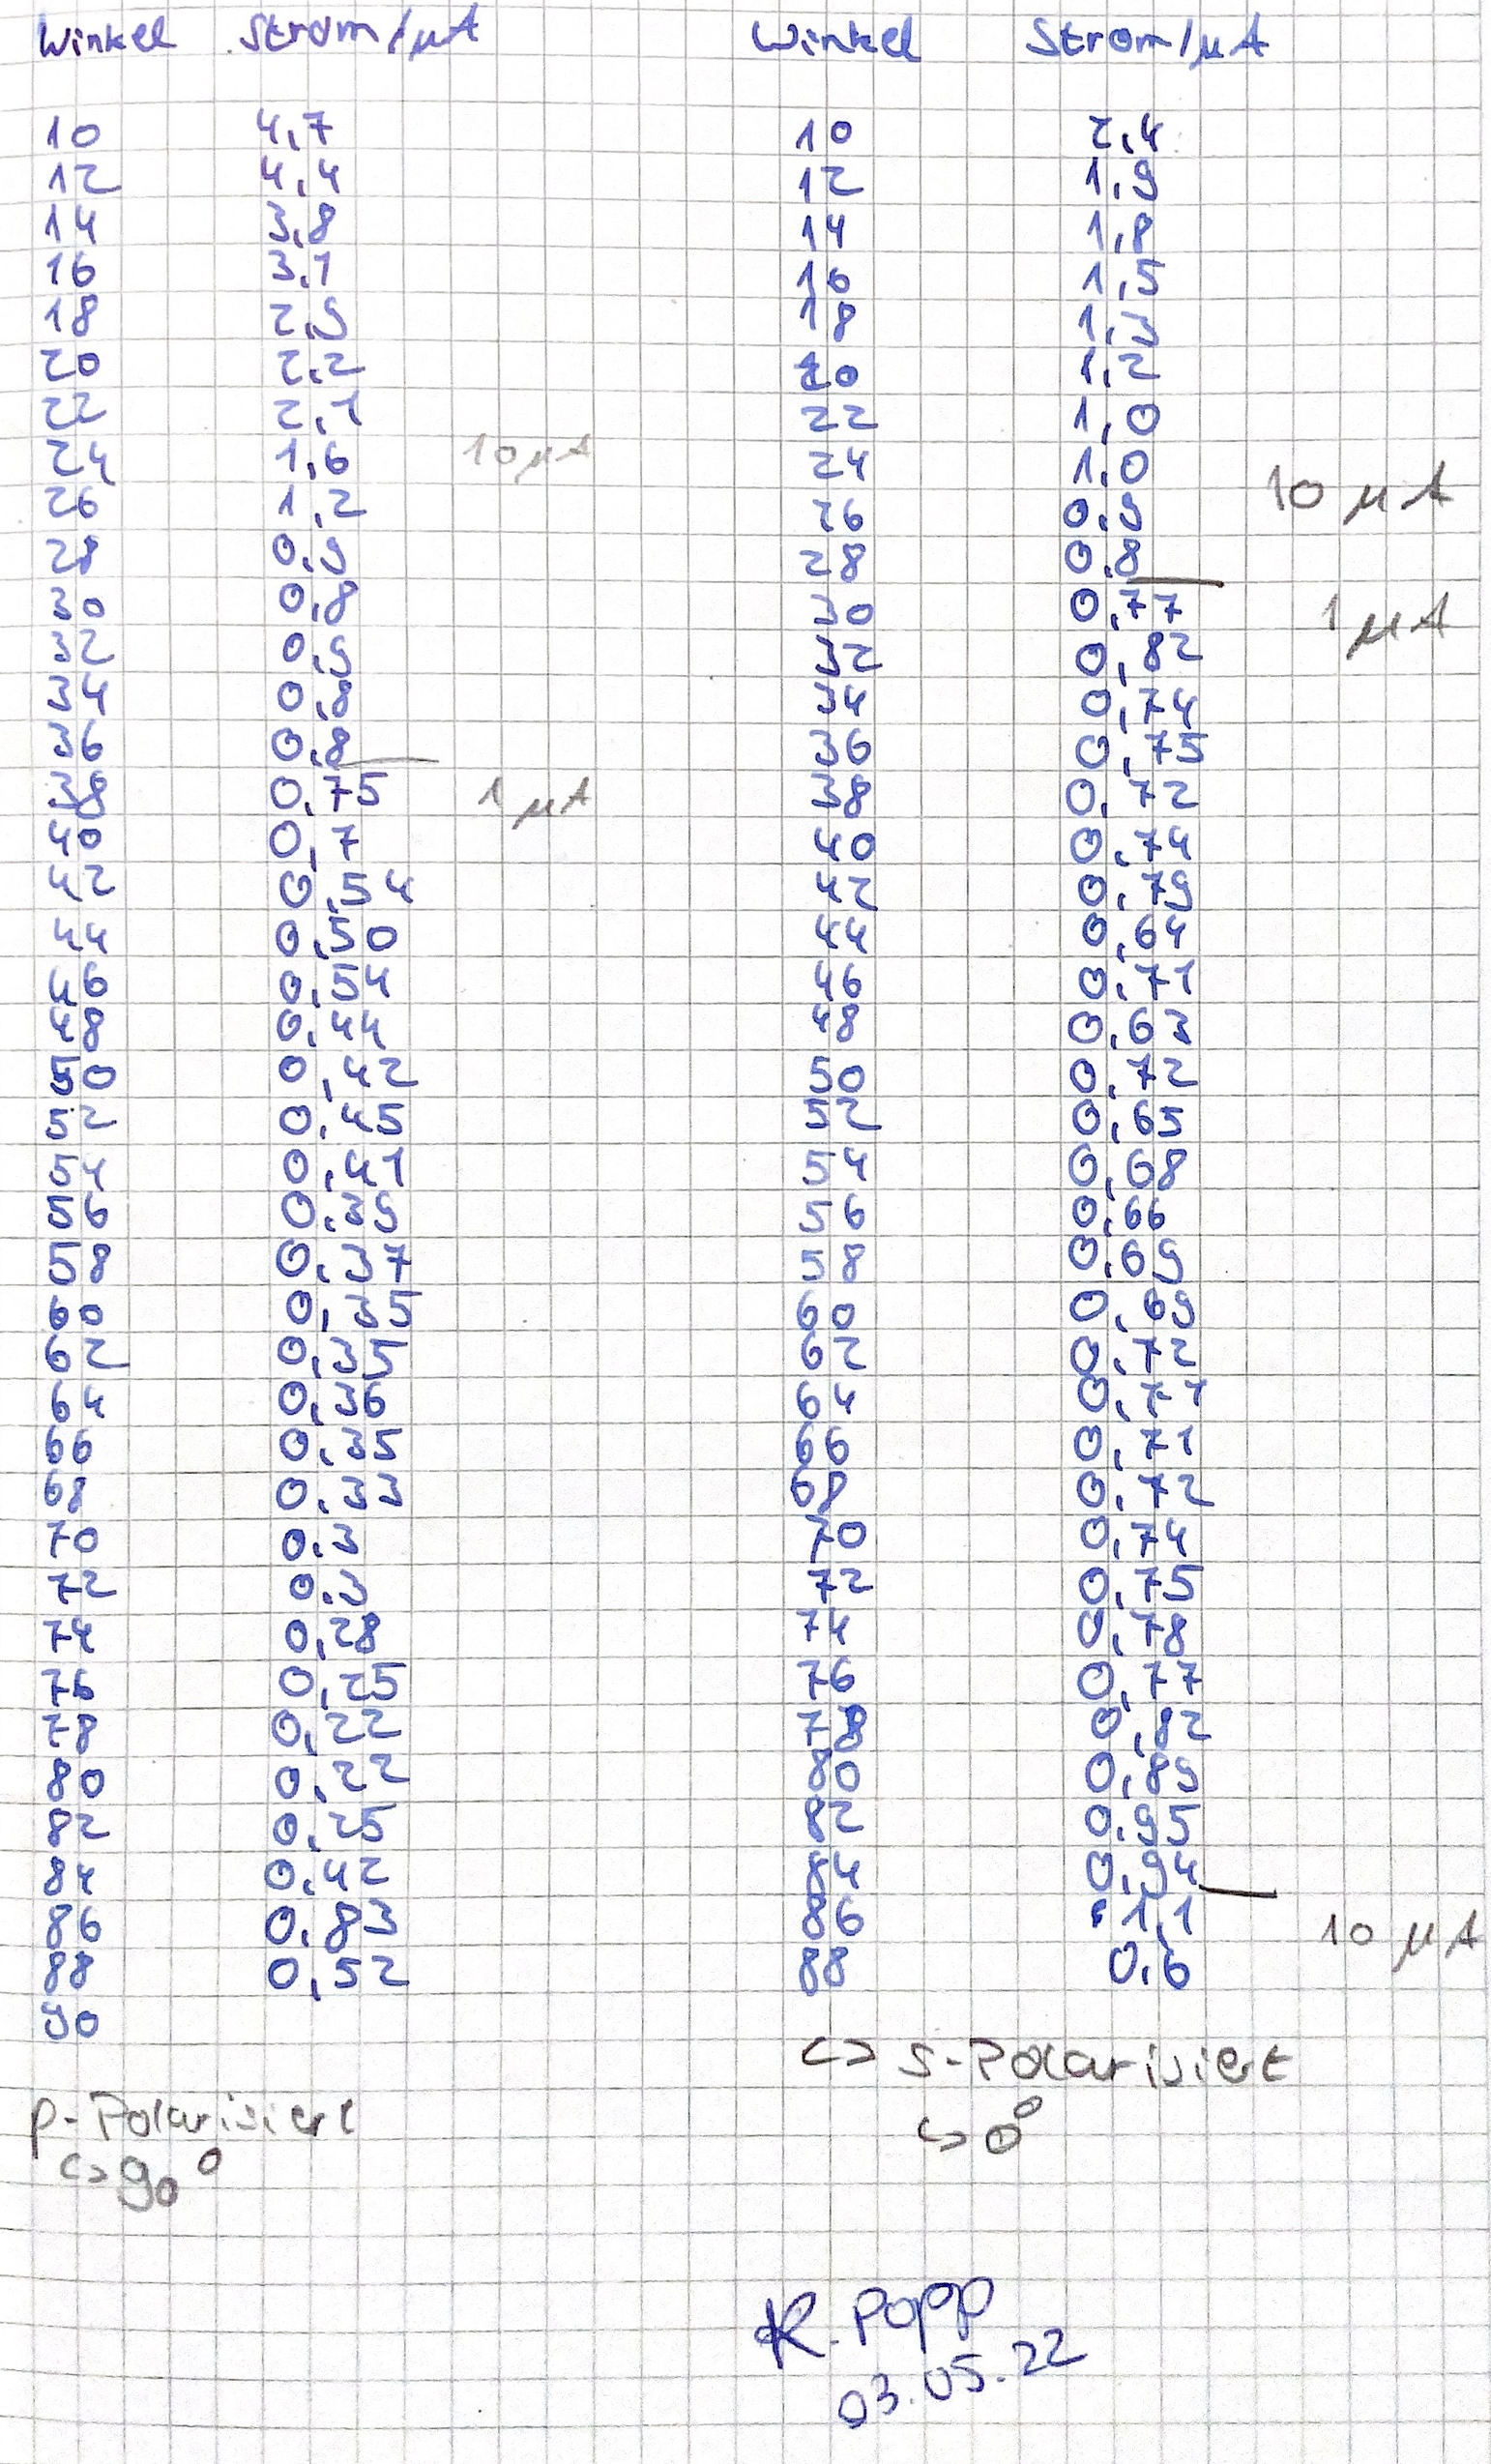
\includegraphics[width=0.75\textwidth]{data/origDaten2.png}
    \caption{Originale Messdaten.}
    \label{fig:origDaten2}
  \end{figure}
}

\end{document}
